\documentclass{beamer}
\usetheme{Boadilla}

\usepackage{amsmath}
\usepackage{amsfonts}
\usepackage{hyperref}

\usepackage{amsmath}
\DeclareMathOperator*{\argmax}{arg\,max}
\DeclareMathOperator*{\argmin}{arg\,min}

\title{Weighted Random Search for Hyperparameter Optimization
}
\author{Galina Boeva}
\institute{MIPT, 2023}


\begin{document}

\begin{frame}
    \titlepage
\end{frame}


\begin{frame}
    \tableofcontents
\end{frame}


\section{Motivation}
\begin{frame}{Motivation}
    \begin{block}{Main idea}
    The motivation is to modernize the generally accepted approaches with an improvement in the quality of work. A weighted search method is proposed, which suggests that a value that has already led to a good result is a good candidate for a new test and should be tested in new combinations of hyperparameter values.
    \end{block} 
\end{frame}


\section{The WRS Method}
\begin{frame}{The WRS Method}
\centering
\begin{figure}
        \centering
        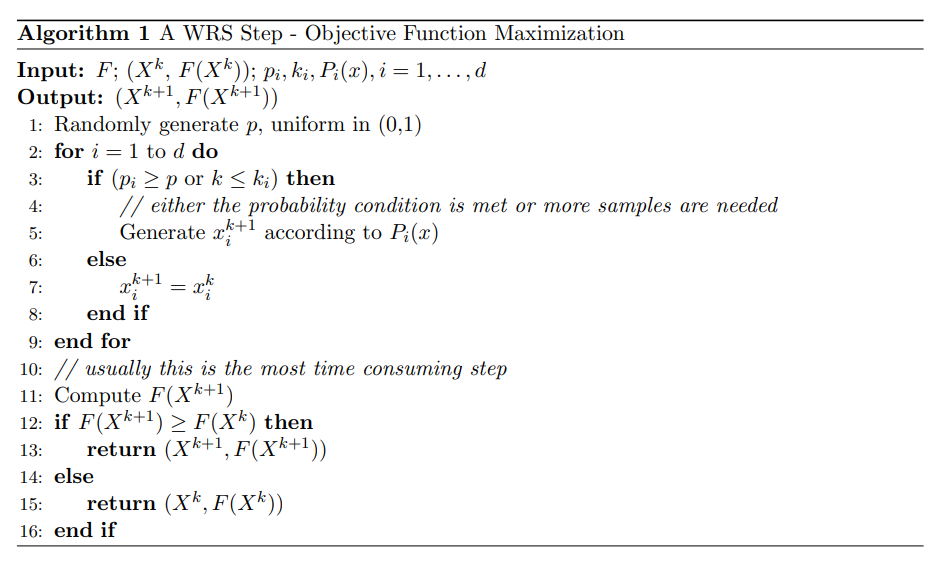
\includegraphics[scale=0.7]{images/wrs.png}
        %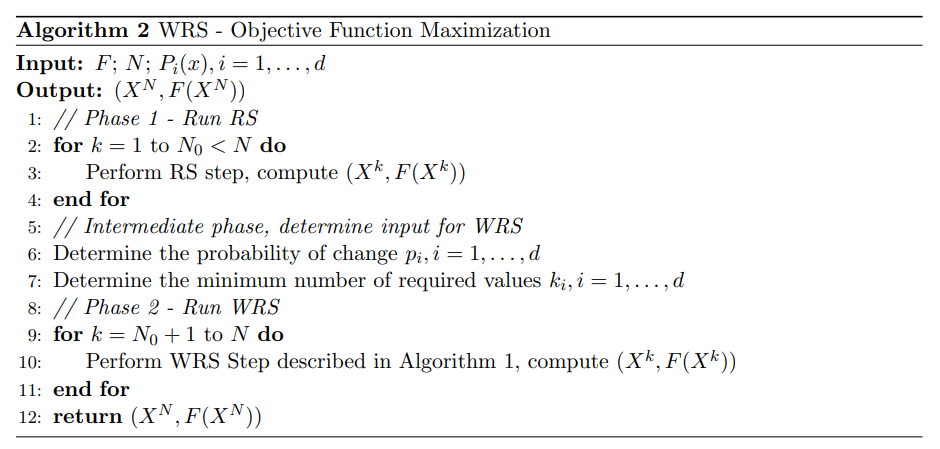
\includegraphics[scale=0.5]{images/wrs2.png}
        \label{fig:enter-label}
    \end{figure} 
\end{frame}

\begin{frame}{The WRS Method}
\centering
\begin{figure}
        \centering
        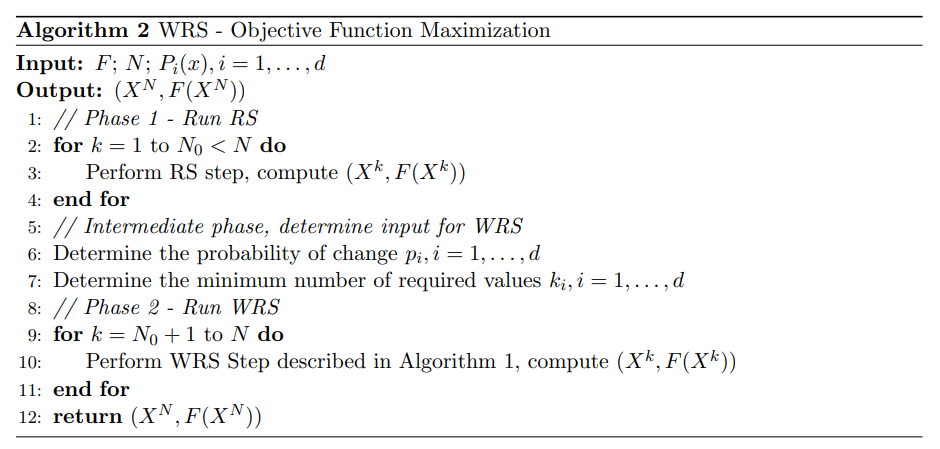
\includegraphics[scale=0.7]{images/wrs2.png}
        %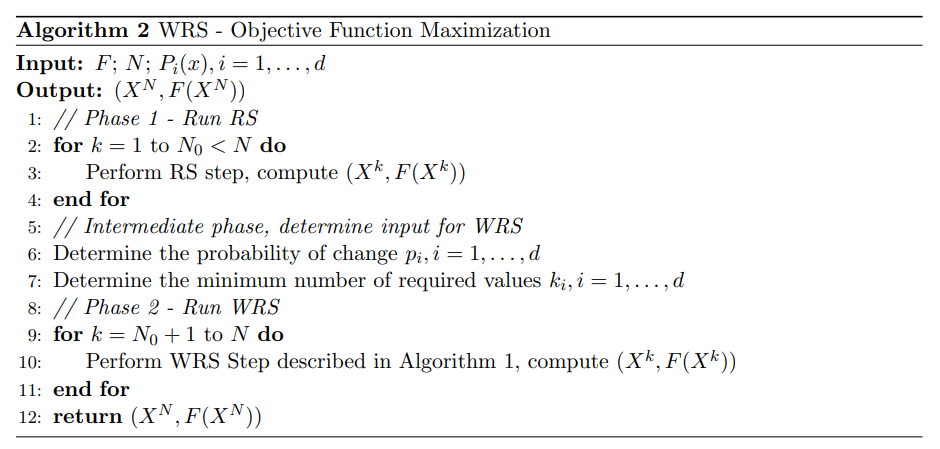
\includegraphics[scale=0.5]{images/wrs2.png}
        \label{fig:enter-label}
    \end{figure} 
\end{frame}

\begin{frame}{Theoretical Aspects and Convergence}
\begin{block}{Multi-dimensional case}
    For the general case of optimizing a function $F : S_1 \times S_2 \dots \times S_d \to R$, with $Si, i = 1, \dots , d$ countable sets and under the same assumption that the variables are not statistically correlated, $P_{RS}$ and $P_{WRS}$ are defined as:
    \[p_{RS} = \prod_{i=1}^d \frac{1}{|S_i|}, p_{WRS} = \frac{1}{|S_1|} \prod_{i=2}^d \left(p_i \frac{1}{|S_i|} + (1 − p_i) \frac{1}{|S_i| - m_i + 1} \right)\]
    where $m_i$ is the number of distinct values already generated for $x_i$.
\end{block}
\begin{block}{Theorem}
    For any function $F : S_1 \times S_2 \dots \times S_d \to R$ there exist $k_i, i = 1, \dots , d$, so that $p_{WRS:n} \geq p_{RS:n}$.
\end{block}
\end{frame}

\begin{frame}{An Example: Griewank Function Optimization}
\centering
\begin{block}{Grievank function}

\[G_d = 1 + \frac{1}{4000}\sum_{i=1}^d x_i^2 - \prod_{i=1}^d \cos\frac{x_i}{\sqrt{i}}\]

We use a slightly modified version of $G_6$, given by:
\[G_6^{*} = 1 + \frac{i - 1}{4000}\sum_{i=1}^6 x_i^2 - \prod_{i=1}^6 \cos\frac{x_i}{\sqrt{i}}\]
\end{block}
\end{frame}
\begin{frame}{An Example: Griewank Function Optimization}
\centering
\begin{figure}
        \centering
        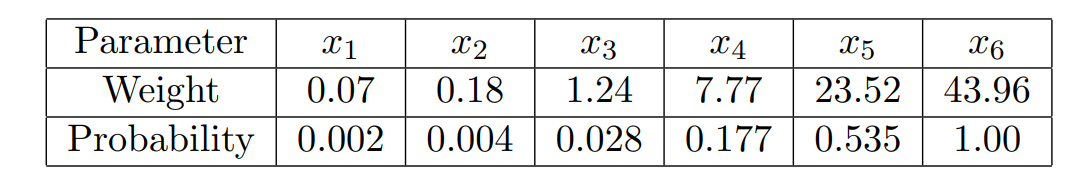
\includegraphics[scale=0.6]{images/wrs3.png} 
        \caption{Parameter weights and probabilities for $G^{*}_6$.}
\end{figure}

\begin{figure}
        \centering 
        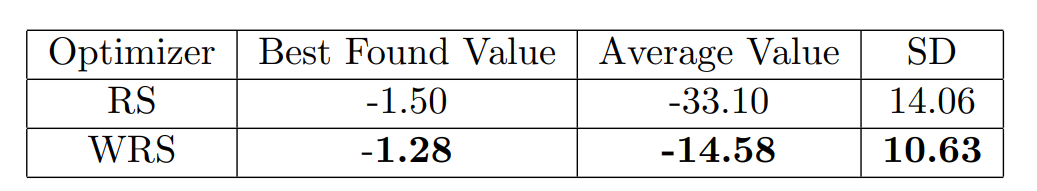
\includegraphics[scale=0.6]{images/wrs4.png}
        \caption{WRS vs. RS results for $G^{*}_6$ - values for 1000 runs.}
\end{figure}
 
\end{frame}

\begin{frame}{An Example: Griewank Function Optimization}
\centering 


\begin{figure}
        \centering
        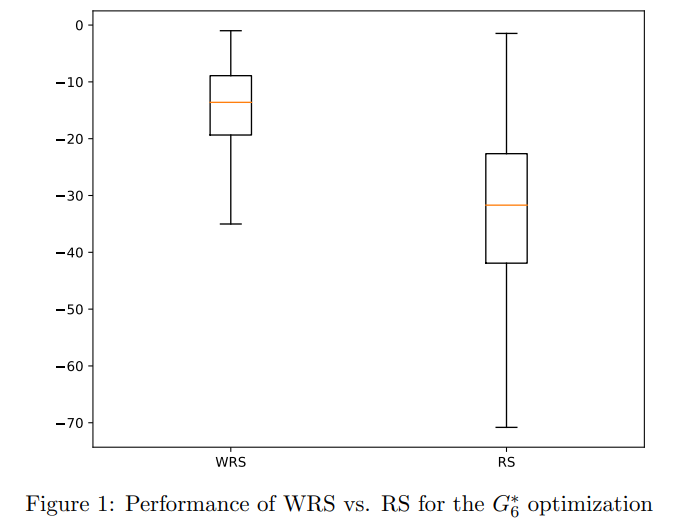
\includegraphics[scale=0.43]{images/wrs5.png}
        \centering
        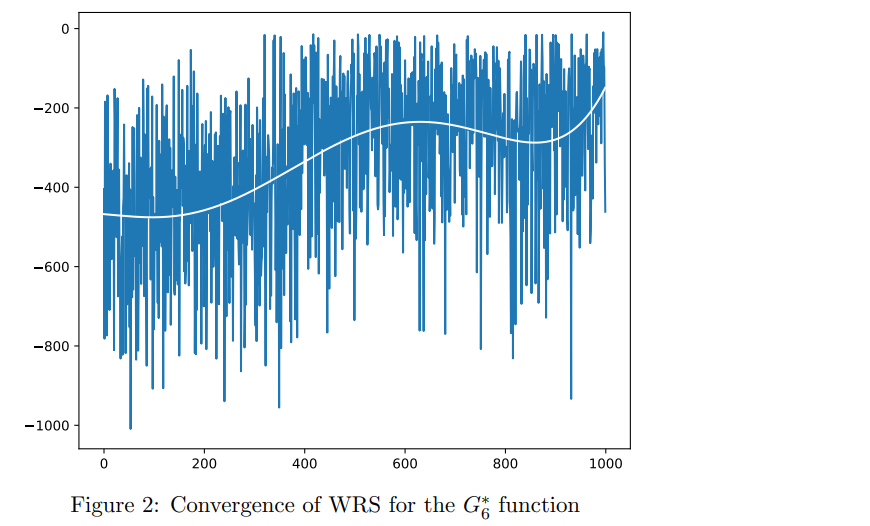
\includegraphics[scale=0.43]{images/wrs6.png}
        \label{fig:enter-label}
    \end{figure}
 
\end{frame}


\section{CNN Hyperparameter Optimization}

\begin{frame}{CNN Hyperparameter Optimization}
    \begin{figure}
        \centering
        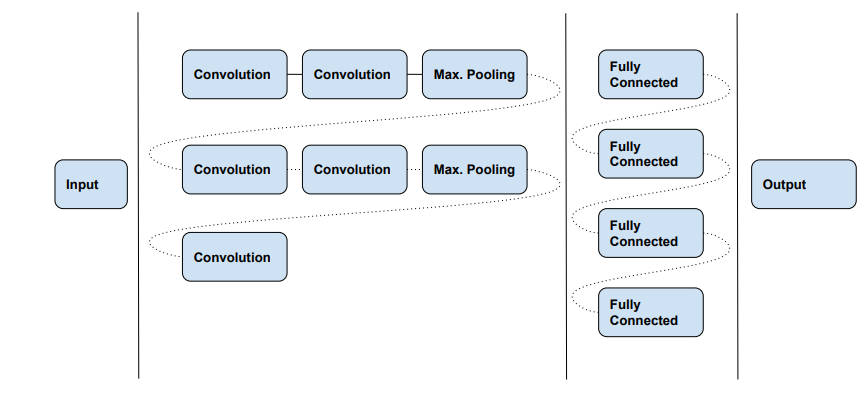
\includegraphics[scale=0.7]{images/wrs7.png}
        \caption{CNN architecture.}
        \label{fig:enter-label}
    \end{figure}
\end{frame}

\begin{frame}{CNN Hyperparameter Optimization}
    \begin{figure}
        \centering
        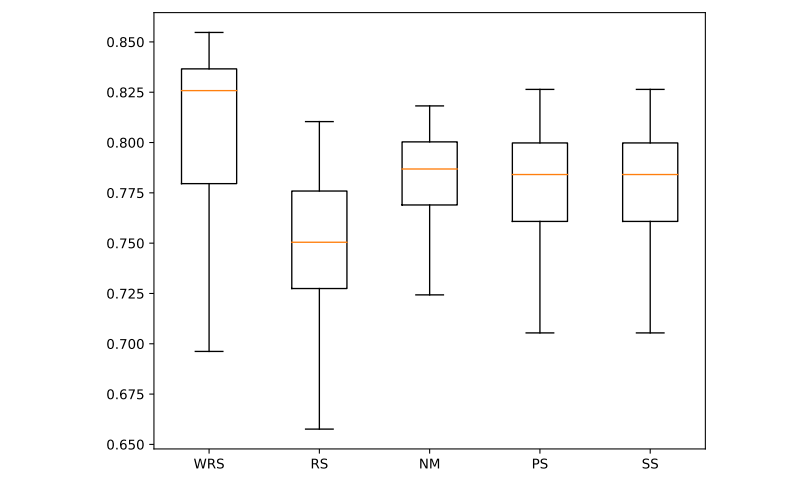
\includegraphics[scale=0.5]{images/wrs8.png}
        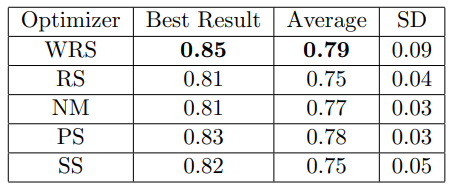
\includegraphics[scale=0.65]{images/wrs9.png}
        \caption{1. Performance of WRS, RS, NM, PS and SS for CNN optimization.
        2. Algorithms’ results for CNN accuracy on CIFAR-10.}
        \label{fig:enter-label}
    \end{figure}
\end{frame}


\begin{frame}{Literature}
    \begin{enumerate}
        \item \textbf{Main article} \href{https://arxiv.org/pdf/2004.01628.pdf}
        {Weighted Random Search for Hyperparameter Optimization}.
    \end{enumerate}
\end{frame}



\end{document}